\section{Video Upload}
\label{sec:video_upload}

This paragraph will illustrate in detail the upload phase of the multimedial contents.
The admin part of the platform allows the selection and the upload of the contents. These operations, however, are contained in a single tag that start the processes shown below.

\begin{lstlisting}[language=html]
   <form class="form">
      <input-s3-video collection="videos" folder="{{folder}}"
        response="{{video}}" error="{{error}}" on-complete="on_response">
      </input-s3-video>
    </form>
\end{lstlisting}

The entire process thats starts with the selection and ends with the content storage on AWS S3 can be synthesized and clarified with the following image:

\begin{figure}[htb]
 \centering
 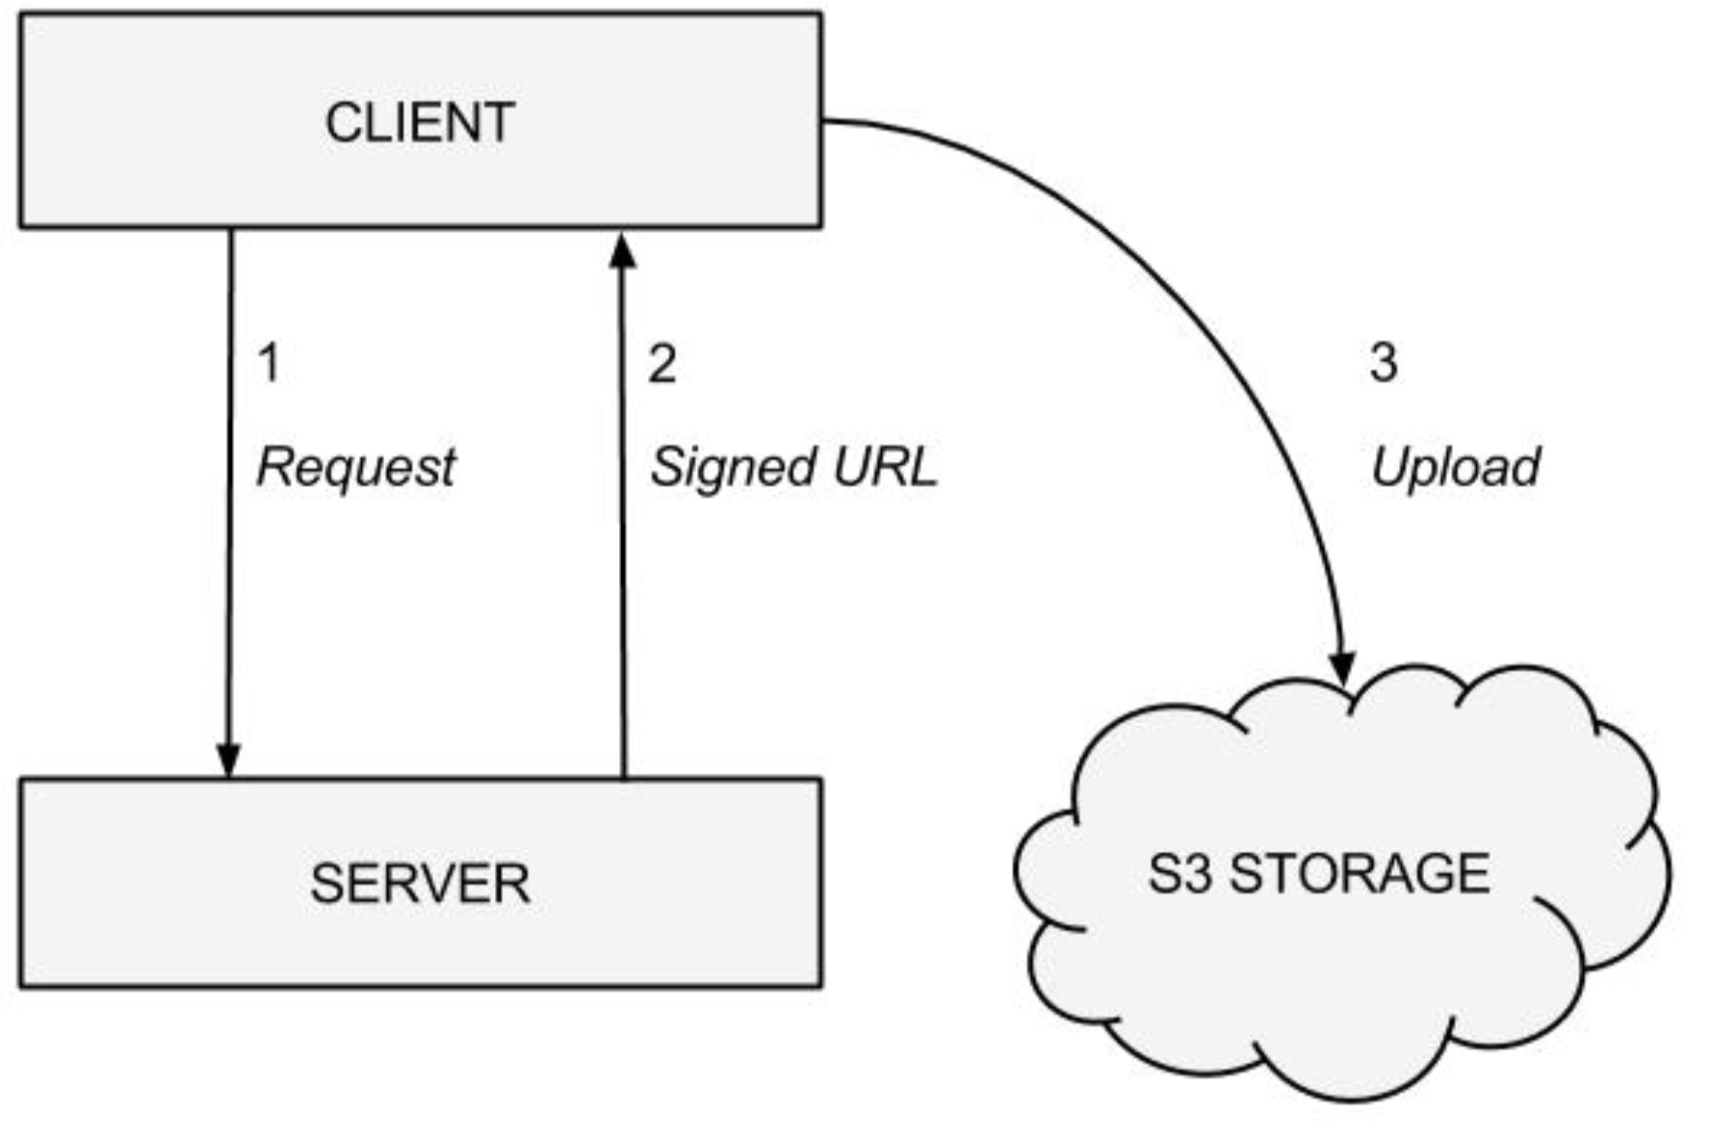
\includegraphics[width=1.0\linewidth]{images/chapter6/upload.png}\hfill
 \caption[Video upload lifecycle]{Video upload lifecycle}
 \label{fig:fourV}
\end{figure}

It can be observed how the upload process is divided in 3 parts:

\begin{enumerate}
\item \textbf{Request}
In the first phase, the communication with Amazon AWS is established, so the client performs a GET operation to the server, passing to it the following information:

   \begin{itemize}
      \item \textbf{params} contains the file name and type
      \item \textbf{url} the API that must be called in this specific case is GET /videos/create\_multiPart\_upload
    \end{itemize}

  \begin{lstlisting}[language=html]
    <iron-ajax id="createMultiPart" method="GET" url="{{url}}" params="{{params}}"
      last-response="{{response_get}}" on-response="on_response_get">
    </iron-ajax>
\end{lstlisting}

The server side through this API calls the following function which allows to establish the connection with AWS and returns the UploadId.
This will be used in the following passages to start a multipart upload.

\begin{lstlisting}[language=javascript]

Video.create_multiPart_upload = function (file_name,file_type,callback){
    var s3_params = {
      Bucket: S3_BUCKET,
      Key: file_name,
      Expires: 6000,
      ContentType: file_type,
      ACL: 'public-read'      
    };
    s3.createMultipartUpload(s3_params, function(err, data) {
      if (err) {
        console.log(err, err.stack); // an error occurred
        callback(err);
        return;
      }else{
        callback(null, data);
      }
    });
  };
  
  Video.remoteMethod('create_multiPart_upload', {
    http: { verb: 'get' },
    accepts: [
      {arg: 'file_name', type: 'string'},
      {arg: 'file_type', type: 'string'}
    ],
    returns: {arg: 'UploadId', type: 'string'}
  });

\end{lstlisting}

Once the AWS response is obtained, client side selected multimedial content is divided into chunks.
The multipart upload can be achieved only with files of dimensions superior to 5MB and because of this, the creation of these chunks relies on a function that:

\begin{itemize}
  \item Check the file dimension
  \item Calculate the number of chunks in a parametric manner based on the dimensions chosen for every chunk
  \item Splits the file in chunks, which will be uploaded on S3 as seen below. 
\end{itemize}


\begin{figure}[htb]
 \centering
 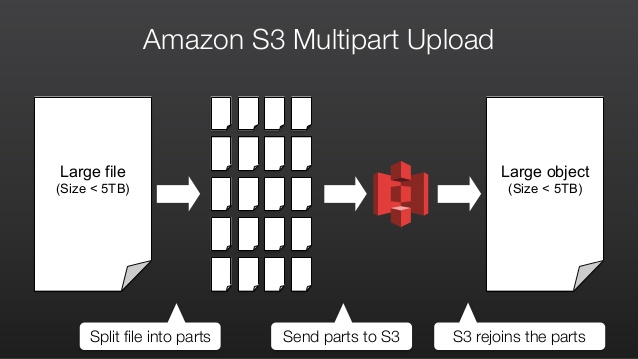
\includegraphics[width=1.0\linewidth]{images/chapter6/multipart.jpg}\hfill
 \caption[Web Components]{AWS MultipartUpload}
 \label{fig:fourV}
\end{figure}

At this point a SignedUrl (phase 2) is requested and uploaded on S3 (phase 3) iteratively for every chunk as seen in the previous figure.

\item \textbf{Signed URL}
  A request is now sent once again to the server through the API GET /videos/signed\_upload\_part.
  Through this API the server function is called, which has the task to ask a Signed Url to AWS, and takes in an input:
  \begin{itemize}
      \item Key is the file name
      \item PartNumber is the i-th chunk that is about to be uploaded
      \item UploadId obtained in the Request phase

  \end{itemize}

\begin{lstlisting}[language=javascript]
  
  Video.signed_upload_part = function(Key,PartNumber,UploadId,callback) {
    var s3_params = {
      Bucket: S3_BUCKET,
      Key: Key,
      PartNumber: PartNumber, /* required */
      UploadId: UploadId /* required */
    };
    s3.getSignedUrl('uploadPart', s3_params, function (err, signed_url) {
      if (err) {
        console.log(err);
        callback(err);
        return;
      }
      callback(null, signed_url);
    });
  };

  Video.remoteMethod('signed_upload_part', {
    http: { verb: 'get' },
    accepts: [
      {arg: 'Key', type: 'string'},
      {arg: 'PartNumber', type: 'number'},
      {arg: 'UploadId', type: 'string'}
    ],
    returns: {arg: 'signed_url', type: 'string'}
  });
\end{lstlisting}

\item \textbf{Upload}
In the third and last phase the Signed Url of AWS is awaited, which will contain the ETAG that represents the id of the i-th chunk.

\begin{lstlisting}[language=html]
var ajax = document.createElement('iron-ajax');
        ajax.url = url;
        ajax.method = 'PUT';
        ajax.body = options.Body;
        ajax.handleAs='json';

        ajax.addEventListener('response', function (event) {
          var xhr = event.detail.xhr;
          var etag = xhr.getResponseHeader('ETag');
          var response = { etag: etag };
          resolve(response);
        });
\end{lstlisting}

As seen in the above snippet, a PUT operation is executed which contains information in the body such as ETAG and the chunk.
Points 2 and 3 described above are executed for every chunk. At the end, the conclusion of the operation is communicated to S3. 
So, client side is called API PUT /videos/complete\_upload\_part which takes the following parameters in input:
  \begin{itemize}
      \item Key is file name
      \item UploadId obtained in Request phase
      \item Parts is an array which contains every chunk id

  \end{itemize}

\begin{lstlisting}[language=javascript]
Video.complete_upload_part = function(Key, UploadId,Parts,callback) {
    var s3_params = {
      Bucket: S3_BUCKET,
      Key: Key,
      UploadId: UploadId,
      MultipartUpload: {
        Parts: Parts
      } 
    };
    s3.completeMultipartUpload(s3_params, function (err, signed_url) {
      if (err) {
        console.log('ERRORE COMPLETE: ' + err);
        callback(err);
        return;
      }

      callback(null, signed_url);
    });
  };

  Video.remoteMethod('complete_upload_part', {
    http: { verb: 'put' },
    accepts: [
      {arg: 'Key', type: 'string'},
      {arg: 'UploadId', type: 'string'},
      {arg: 'Parts', type: 'array' }
    ],
    returns: {arg: 'signed_url', type: 'string'}
  });

\end{lstlisting}

\end{enumerate}
The upload can be considered terminated only at the end of this operation. AWS will then reconstruct the file by uniting all the chunks received and specified in the Parts section of the previous function.